%!TeX spellcheck = en-US
\documentclass[../main.tex]{subfiles}
\begin{document}
\chapter{Scenario}
\label{chap:avionicsprot}

The technological explosion of the last years influenced also the aviation sector. Better planning, more efficient planes and many other management improvements brought the price of airline tickets down making traveling by plane accessible to anyone. More recently the drone market rapidly grew to the point where every professional and amateur video maker must have at least one drone to capture great aerial shots that in the past could only be done with the use of an helicopter. Moreover companies like \textit{Amazon} and \textit{DHL} successfully tested a parcel delivery service operated by drones\cite{primeair} while other companies like \textit{Facebook} and \textit{Google} started testing an affordable and reliable method to bring internet connection to remote areas of the planet\cite{loon}. All this sudden progress lead to an overcrowding of the skies to which the innovation in the  \textbf{\acrlong{atm}} (\textbf{\acrshort{atm}}) field must keep up.

We can no longer see just airplanes as the main users of the sky but We must consider a wider spectrum of objects since nowadays flying objects are quite heterogeneous: aircraft alone are divided into different categories depending on the maximum altitude, their weight and other parameters. Commercial drones like the ones from \textit{Amazon} or the cinematography ones are starting to have capabilities similar to a small aircraft in term of performance. On the other hand \textit{Facebook} Aquila drones have the same wingspan as a Boeing 737 and they fly at a considerably high altitude\cite{fbaquila}. Also Project Loon internet balloons travel at high altitude and trough busy airspace. In addition to those there are many other objects like gas balloons, helicopters and gliders operating in certain areas and airspace class that must be tracked, managed and monitored efficiently to ensure high safety standards.

For this reasons and to overcome the absence of radar coverage in certain areas of the planet (e.g over the ocean) a modernization of the radar and communication system was launched starting from the 80s up to the present days with the development of two generations of protocols. Different organizations collaborate in defining the standards and guidance documents for aeronautics, the major of which are \acrlong{rtca} (\textbf{\acrshort{rtca}}) in the United States, \acrlong{eurocae} (\textbf{\acrshort{eurocae}}) in Europe and \acrlong{icao} (\textbf{\acrshort{icao}}) which is a United Nations organization. All those organizations are non governative therefore they produce standards, guidelines or rules that will then have to be adopted by the \acrlong{faa} (\textbf{\acrshort{faa}}) in the united states, by the \textbf{EUROCONTROL}\footnote{Organization to provide unique centralized platform for civil and military aviation coordination in Europe.} and the single national aviation authority of the various European countries (\textit{\acrshort{enac}/\acrshort{enav}} in Italy). This fragmentation of the organizations, the absence of a globally shared guidance on the standardization of the aviation sector (which is partially an \acrshort{icao} task.\footnote{Art 1. The contracting States recognize that every  State has complete and exclusive sovereignty over the airspace above its territory.\cite{icao7300}}) and the development of different standards to accomplish the same task brought to an unclear situation regarding standards and regulations especially in the NextGen where there were some problems in the definition of a globally accepted family of protocols as it can be seen in the appropriate section.

Aircraft can be tracked in two ways, a \textbf{cooperative} one and a \textbf{non-cooperative} one:

\begin{itemize}

  \item The classic radar (or Primary Radar), based on electromagnetic waves is able to give information only on the position of an object in the sky. Such system gives a real-time image of the portion of sky that it is observing, this includes aircraft, birds, clouds, and any other object in his field of view making it a basic and fairly unreliable system. Since this method requires no interaction with the aircraft that is being traced, for this reason it is called \textbf{non-cooperative} system.
  \item \acrlong{ssr} (\textbf{\acrshort{ssr}}) is an evolution of the above system which, in addition to the spatial position of the aircraft, gives additional information depending on his mode of operation. Since this system requires an active cooperation from the aircraft which must reply to the interrogations send by the system which makes it a \textbf{cooperative} system.

\end{itemize}

The cooperative systems allow having a bidirectional aircraft-ground as well as aircraft-aircraft data flow. This system stems from the military \acrlong{iff} (\textbf{\acrshort{iff}}) one which was developed during the Second World War. The actual civil system uses a 4 digit code called "Transponder Code" or \textbf{"Squawk"} to identify the aircraft, this communicates via a \textbf{transponder} which handles the incoming interrogations and the responses. In Figure \ref{fig:allgen} is an overview of all the protocols and their division between the old generation and the new generation which is still in deployment.

Having a continuous data flow between the aircraft and the ground is beneficial not only for the \acrshort{atm}/\acrshort{atc} but also for the airline. In fact:
\begin{itemize}
  \item Flight controllers can obtain much more information about a single aircraft, his intentions and the status of the flight. Moreover satellite based ADS-B allows tracing planes in areas where no radar coverage is available.
  \item The airline can keep track of his fleet in real time thus allowing a better planning of the turnover and,if needed, quick deployment of a replacement airplane.
  \item The maintenance branch of the airline can track in real time any anomalies reported by the aircraft instruments and sensors performing a remote analysis and helping the pilots in the troubleshooting process allowing them to take better decisions.
\end{itemize}

As previously mentioned the current avionics protocols can be divided in two families: \textbf{OldGen} and \textbf{NextGen}. The \textbf{OldGen} is currently deployed and used globally while the \textbf{NextGen} is standardized an set to be fully deployed by 2020. For this reason, to comply with regulations and to enhance safety Project Loon balloons are equipped with both OldGen and NextGen hardware\cite{loonadsb} while some DJI drones are compatible with NextGen protocols\cite{dji}.

\begin{figure}[htp]
  \centering
  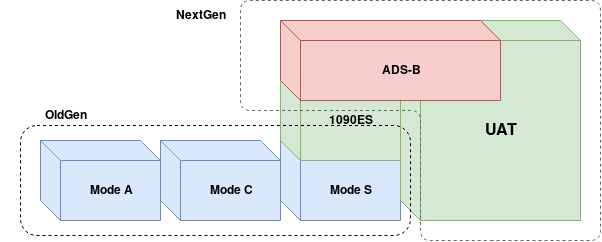
\includegraphics[scale=0.6]{images/allgen.png}
  \caption{All generation of avionics protocols}
  \label{fig:allgen}
\end{figure}

\section{OldGen}

The first generation of protocols is fairly simple, it uses the 1030MHz frequency for interrogation while the 1090MHz frequency is used for replies.
The first two protocols are \textbf{Mode A} and \textbf{Mode C}.

\textbf{Mode A} is the simplest, it responds to an interrogation request just by broadcasting the \textbf{squawk} code which was previously assigned to the pilot by the controller. In this way the controller can identify the aircraft on his screen by such code. In addition to this the pilot can manually generate a special response called \textit{"Ident"} or \textit{"\acrshort{spi}"} (\acrlong{spi}) which is used to highlight the aircraft on the controller screen.

\textbf{Mode C} is an extension of the previous protocol which, in addition to the transponder code, sends information about the altitude and the pressure. This kind of transponders are often referred as \textbf{Mode A/C} transponder.

\textbf{Mode S} is the newest protocol and it is an hybrid between the two generations. It is backward compatible with the \textbf{Mode A/C} but at the same time it is also part of the NextGen as it can be seen in Figure \ref{fig:allgen}. \textbf{Mode S} ground stations and transponders support both all call interrogations and selective interrogation, in particular each aircraft is identified by a unique 24-bit address which is part of the aircraft registration documents and should never change. The address is transmitted with every \textbf{Mode S} reply. In this way a \acrshort{ssr} station can perform an all call interrogation to acquire each aircraft address which can then be used to selectively interrogate them. To identify each ground station a 4-bit\footnote{For aircraft complying with ICAO Annex 10, Volume IV Amendment 73 a 6-bits code can be used} \acrlong{ic} (\acrshort{ic}) is used. In this way single aircraft interrogation as well as lock-out of the aircraft can be performed in order to avoid multiple pickups of the same aircraft by different \acrshort{ssr} stations. \textbf{Mode S} messages can be of 56 or 112 bits and they are structured as in Figure \ref{fig:modes}.

\begin{figure}[htp]
  \centering
  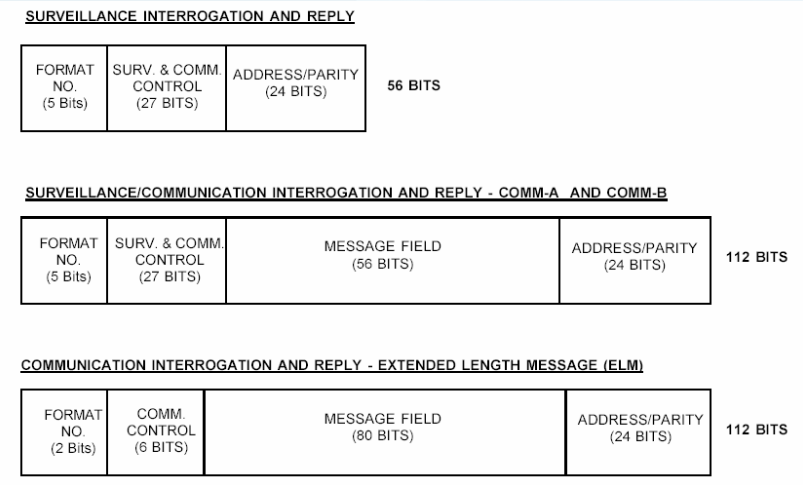
\includegraphics[scale=0.65]{images/modes.png}
  \caption{Mode S messages}
  \label{fig:modes}
\end{figure}

The above protocols are at the base of the \acrlong{acas} (\textbf{\acrshort{acas}}). This system requires both aircraft to be equipped with \textbf{Mode A/C}, \textbf{Mode C} or \textbf{Mode S} transponders. In this way it can keep track of the surrounding airplanes and, in case of colliding traffic, propose vertical \acrlong{ra} (\textbf{\acrshort{ra}}). NextGen systems have enhanced \textbf{RA} capabilities. It is clear that this is a critical part of the system and, if compromised, can lead to dramatic results such as mid air collision.

\textbf{Mode A/C} and \textbf{S} are the current standards and they are widely used, for example: according to the Italian regulation all aircraft must be equipped with at least a \textbf{Mode A/C} transponder and in some particular case with a \textbf{Mode S} transponder as it can be seen in GEN 1.5-3.1 of AIP Italia\cite{itareg}.

Beside the basic protocols that we described here there is a more sophisticated one that lays between the two generations.
The \acrlong{acars} (\textbf{\acrshort{acars}}) is in use since the 1978, at first it relayed only on \acrshort{vhf} radio channels but in the years has been improved to add other transmission means to expand coverage. It is also now deeply integrated into the aircraft systems giving it access to a large number of data and the ability to operate autonomously. Acars messages can be delivered via 3 different transmission means: \acrshort{vhf} Data Link, \acrshort{hf} Data Link and satellite. Depending on the position one method can be better than another, for example \acrshort{vhf} works only in line of sight while satellite communication (SATCOM) is not available at the poles. \textbf{\acrshort{acars}} messages can be of 3 different types:
\begin{itemize}
  \item \acrlong{atc} messages. Used in some busy airports as an alternative to the radio. And in routes where no radio contact is possible (e.g oceanic routes).
  \item Aeronautical Operational Control (AOC) and Airline Administrative Control (AAC) used to send documents to the aircraft as well as to receive error messages or information on the status of the flight.
  \item Free Text Message
\end{itemize}
Messages from aircraft can be pre-configured so that they are automatically delivered to the appropriate recipient based on the message type, in the same way ground-originated messages can be configured to reach the correct aircraft. This messages covers a fundamental part of the bidirectional aircraft-ground data link and their content can be of utmost importance.
For example the Air France flight 447 which disappeared from the radars on 1 June 2009 sent in his final moments 24 \textbf{\acrshort{acars}} messages some of them indicating anomalies and errors. In the first moments those messages where the only clue to understand what happened and to locate the aircraft \cite{af447}.
\bigskip

\section{NextGen and SESAR}

Both \textbf{NextGen} and \textbf{\acrshort{sesar}} (\acrlong{sesar}) are efforts to modernize the air transportation system respectively from the United States government and from the European Union along with other private parties. Both programs aims to achieve a higher degree of safety enhancing communications, navigation, surveillance technologies thus enabling all the users of the sky, even the future one, to virtually see each other. The introduction of those new standards will also bring a reduction of costs through better \acrshort{atm} and enabling low visibility operations. The efforts are coordinated in order to assure a globally accepted common standard, for this reason from now on I will not make any distinction and refer to both protocols as \textbf{NextGen}. However under the \textbf{NextGen} family goes many different protocols and some of them are not shared between Europe and America even if there are plans to do that.

The main component of this system is \acrlong{ads-b} (\textbf{\acrshort{ads-b}}).
\textit{"The American Federal Aviation Administration (FAA) as well as its European counterpart EUROCONTROL named ADS-B as the satellite-based successor of radar."}\cite{stroh14}
\textbf{\acrshort{ads-b}} is an automatic system which broadcasts aircraft sensors information to the outside world. It is divided in "ADS-B Out" which requires just a transponder able to properly encode messages and "ADS-B In" which requires a receiver, a computer and an interface to display the data.
\textbf{\acrshort{ads-b}} messages are also picked up by ground stations which feeds the data to a central system where they are used, in combination with other data (e.g radars), to create a Traffic Situation Picture.

Two main protocols where proposed to deliver \textbf{\acrshort{ads-b}} messages:
\begin{itemize}
  \item \textbf{1090ES} (Extended Squitter)
  \item \textbf{\acrshort{uat}} (\acrlong{uat})
\end{itemize}

\textbf{1090ES} it is the current global standard for \textbf{\acrshort{ads-b}} in commercial aviation. In Europe 1090ES is required for \acrshort{ifr} aircraft with a \acrshort{mtow} exceeding 12,566 pounds or maximum cruise airspeed faster than 250 KTAS. All aircraft must complain with this regulation by 2020. \cite{eu1090}

In USA \textbf{1090ES} will be mandatory for all aircraft after June 2020 and is the only technology that should be used when flying above 18 000 feet.
\cite{title14}. An overview of the USA supported technologies in the various airspace can be seen in Figure \ref{fig:uatvs1090}

This protocol is backward compatible with the \textbf{OldGen} since it uses the same frequencies and, in particular, a transponder supporting \textbf{Mode S} messages can be easily updated to \textbf{\acrshort{ads-b}}. In fact \textbf{\acrshort{ads-b}} information are simply carried inside a 112 bit \textbf{Mode S} message as it can be seen in Figure \ref{fig:1090es}.


\begin{figure}[htp]
\centering
\begin{minipage}{.5\textwidth}
  \centering
  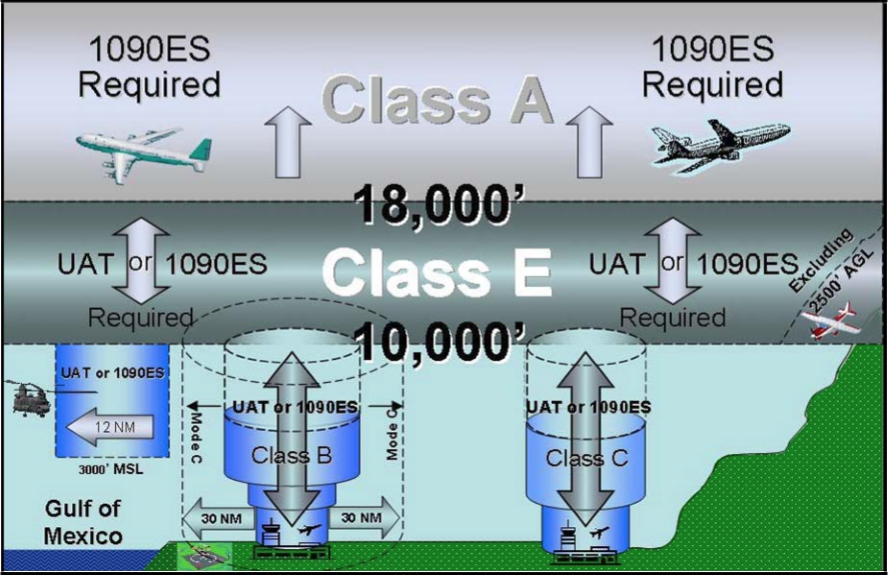
\includegraphics[scale=0.35]{images/uatvs1090.png}
  \caption{USA airspace}
  \label{fig:uatvs1090}
\end{minipage}%
\begin{minipage}{.5\textwidth}
  \centering
  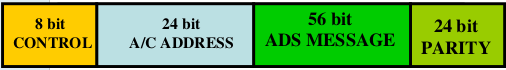
\includegraphics[scale=0.45]{images/1090es.png}
  \caption{1090ES Message}
  \label{fig:1090es}
\end{minipage}
\end{figure}

\textbf{\acrshort{uat}} although in the name it says Universal Access it is not yet widespread as \textbf{1090ES}. This protocol is mainly deployed in North America and it is starting to be deployed also in China. It is not backward compatible with the \textbf{OldGen} and it was developed specifically to be used with \textbf{ADS-B}. It uses the 978MHz frequency and requires an entire new hardware to work.

However since it is a newly designed protocol built to be future proof it allows to carry more information compared to \textbf{1090ES}, such as weather reports, pilots reports and other messages using the \textbf{\acrshort{fis-b}} (\acrlong{fis-b}) and \textbf{\acrshort{tis-b}} (\acrlong{tis-b}). Those are ground services that broadcasts to "ADS-B In" equipped aircraft information on weather and traffic detected by ground radars as well as coming from other ADS-B equipped planes. Moreover \textbf{\acrshort{fis-b}} service is also capable to deliver \textbf{NexRad} images captured from the United States Weather Surveillance Radar through \textbf{ADS-B} messages. US government is encouraging General Aviation (GA) aircraft, not flying in Class A airspace, to use a \textbf{UAT} transponder. In this way there is less pollution of the 1090MHz frequency and they can receive more information such as weather data.

\textbf{NextGen} protocols will also substitute a big part of the voice communications not only between pilots and air traffic control but also between air traffic controllers themselves using the \textbf{\acrshort{uat}} data link and the previously mentioned \textbf{\acrshort{acars}} messages.
In particular \textbf{\acrshort{ads-c}} (\acrlong{ads-c}) automatically aggregate data such as aircraft position, altitude, speed, intent and meteorological data from onboard sensors. The generated report can then be sent to an ATS (\acrlong{ats}) unit or \acrshort{aoc} (\acrlong{aoc}) facility ground system for surveillance and route conformance monitoring \cite{goldman}. An \acrshort{ats}  ground station must authenticate on the aircraft system to require a contract. Contracts can be of 3 types:

\begin{itemize}
  \item Periodic: the \acrshort{ats} specify the time interval at which the aircraft sends the report.
  \item Demand: is a single report requested from the ground station. This request does not affect any other contracts that might be present.
  \item Emergency: this reports are tagged as "emergency" report and will be highlighted to the \acrshort{atc}. Emergency reports can be generated manually by the crew or as a consequence of triggering another type of emergency system.
  \item Event: the \acrshort{ats} unit can specify the event (limited to 1 per aircraft) at which the report will be send. The contract can contain multiple event types (e.g lateral deviation, vertical rate change ecc).
\end{itemize}
\end{document}
